% % % % % % % % % % % % % % % % % % % % % % % % % % % % % % % % % % % % % % % %
% LaTeX4EI Template for Cheat Sheets                                Version 1.1
%
% Authors: Markus Hofbauer
% Contact: info@latex4ei.de
% Encode: UTF-8
% % % % % % % % % % % % % % % % % % % % % % % % % % % % % % % % % % % % % % % %


% ======================================================================
% Document Settings
% ======================================================================

% possible options: color/nocolor, english/german, threecolumn
% defaults: color, english
\documentclass[german, 8pt]{latex4ei/latex4ei_sheet}

% set document information
\title{Physik}
\author{LaTeX4EI}                    % optional, delete if unchanged
\myemail{info@latex4ei.de}           % optional, delete if unchanged
\mywebsite{www.latex4ei.de}          % optional, delete if unchanged

%custom settings
\titlespacing*{\subsection}{.5pt}{.5pt}{2pt}
\titlespacing*{\subsubsection}{0pt}{.5pt}{2pt}

% ======================================================================
% Begin
% ======================================================================
\begin{document}

% Title
% ----------------------------------------------------------------------
\maketitle   % requires ./img/Logo.pdf


% Allgemein
% ----------------------------------------------------------------------
\section{Allgemeines}

% Klassische Mechanik
% ----------------------------------------------------------------------
\section{Klassische Mechanik}
\subsection{Bewegungen}
\subsubsection{Freier Fall}
\subsubsection{Ebene}
\subsubsection{Senkrechter Wurf}
\subsubsection{Waagrechter Wurf}
\subsubsection{Schräger Wurf}
\subsection{Newton'sche Axiome}
\subsection{Kraft, Energie, Impuls}
\subsubsection{Kraft}
\subsubsection{Arbeit}
\subsubsection{Leistung}
\subsubsection{Energie}
\subsubsection{Impuls}
\subsubsection{Raketengleichung}
\subsection{Planetenbewegungen}
\subsubsection{Gravitation}
\subsubsection{Keplersche Gesetze}
\subsection{Drehungen}
\subsubsection{Drehmoment}
\subsubsection{Trägheitsmoment}
\subsubsection{Drehimpuls}
\subsection{Corioliskraft}
\begin{emphbox}
$\vec{F_c}=2m(v\times \omega)= 2m \cdot v \cdot w	\cdot \sin{(v\angle \omega)}$
\end{emphbox}
$a_c=-2(\omega \times v)=2v\omega$\\
$\Delta x= \frac{2}{3}\cos \beta \omega h \sqrt{\frac{2h}{g}}$\\
$\Delta y = -\omega^2R\cos \beta \sin \beta \frac{h}{g}$\\
Rechte-Hand-Regel: Daumen: $\vec{v}$, Zeigefinger: $\vec{\omega}$ (von Süden nach Norden)\\
%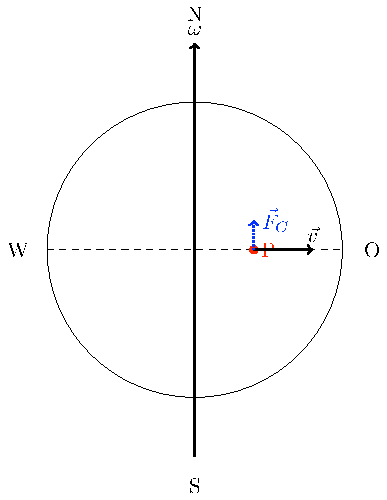
\includegraphics[width=0.25\columnwidth]{coriolis.pdf}
$R_E=\SI{6370}{\kilo \meter}$\\
$r=R_E \cos \varphi$
$\omega_E=\frac{2\pi}{86400\si{\second}}$\\
Auf der Nordhalbkugel zeigt $F_C$ nach rechts. Auf der Südhalbkugel nach links.


% Harmonische Schwingungen
% ----------------------------------------------------------------------
\section{Harmonische Schwingungen}
\subsection{Frei ungedämpft}
\subsubsection{Federpendel}
\subsubsection{Fadenpendel}
\subsubsection{Torisionsschwingungen}
\subsection{Frei gedämpft}
\subsubsection{Fälle}
\subsection{Erzwungen gedämpft}
\subsubsection{Resonanzfälle}

% Wellen
% ----------------------------------------------------------------------
\section{Wellen}
\subsection{Allgemeines}
\subsection{Doppler-Effekt}
\subsection{Schwebung}
\subsection{Gekoppelte Wellen}
\subsection{Interferenz}
\subsubsection{Doppelspalt}
\subsection{Reflexion/Wellen in einem Medium}

% Optik
% ----------------------------------------------------------------------
\section{Optik}
$f_m \cdot \lambda_m = c_m$ \qquad
$\lambda_m = \frac{\lambda_0}{m}$\\
Berchnungsindex $n=\frac{c_0}{c_m}$
\subsection{Rexlexion und Brechnung}
\subsubsection{Brechung}
\begin{enumerate}
\item[A)] zum Lot (dünn nach dicht)\\
$\sin \alpha > \sin \beta$ \qquad $c_1 > c_2$
\item[B)] vom Lot (dicht nach dünn)\\
$\sin \alpha < \sin \beta$ \qquad $c_1 < c_2$
\end{enumerate}
\subsubsection{Gesetz von Snellius}
$\frac{\sin \alpha}{\sin \beta} = \frac{n_2}{n_1} = \frac {c_1}{c_2}$
\subsubsection{Totalreflexion}
Nur möglich wenn $n_1 > n_2$ und $\theta > \theta_{\ir krit}$ \\
$\theta_{\ir krit} = \arcsin \frac{n_2}{n_1}$\\
Einfallswinkel = Ausfallswinkel
\subsection{Linsen}
Linsengleichung
\begin{emphbox}
$D=\frac{1}{f}=\frac{1}{g}+\frac{1}{b}$	
\end{emphbox}
Vergößerung: $V=\frac{B}{G}= - \frac{b}{g}=\frac{\tan \alpha}{\tan \alpha_0}$\\
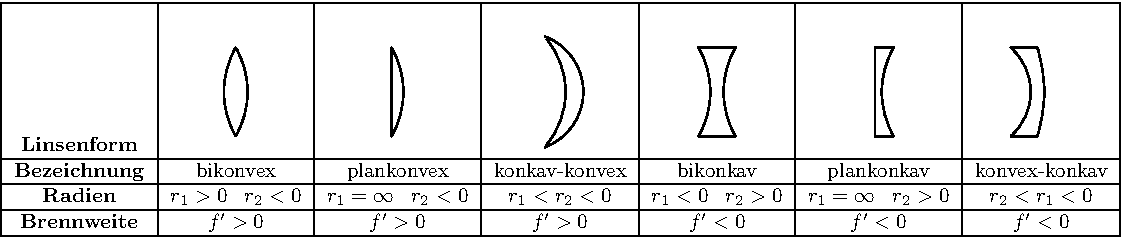
\includegraphics[width=\columnwidth]{img/Linsen_crop.pdf}
\subsubsection{Hohlspiegel}
$f=\frac{r}{2}$ \qquad $V=\frac{B}{G}= - \frac{n_1b}{n_2g}$ \\
$D=\frac{n_1}{g}+\frac{n_2b}=\frac{n_2-n_1}{r}$\\
$g\rightarrow \infty: b=f_B=\frac{n_2r}{n_2-n_1}$\\
$b\rightarrow \infty: g=f_G=\frac{n_1r}{n_2-n_1}$\\
%Bild
\subsubsection{Dünne Linsen}
$\frac{1}{f}=\frac{1}{g}+\frac{1}{b}=(\frac{n_2}{n_1}-1)(\frac{1}{r_1}-\frac{1}{r_2})$
\textbf{Konvexe Linse (Sammellinse)}
$V_{\ir sammel}= \frac{b}{g}=\frac{b-f}{f}$\\
Korrektur von Weitsichtigkeit \\
%Bild
\textbf{Abbildung}
\begin{itemize}
	\item $\infty > g > 2f \Rightarrow 2f>b>f \quad G>B$ (real und invertiert)
	\item $g=2f \Rightarrow 2f=b \quad G=B$ (real und invertiert)
	\item $2f>g>f \Rightarrow \infty >b>2f \quad G<B$ (real und invertiert)
	\item $0<g<f \Rightarrow -b>g \quad G<B$ (virtuell und aufrecht)
\end{itemize}
\textbf{Konkave Linse (Zerstreuungslinse)}
Korrektur von Kurzsichtigkeit\\
\textbf{Abbildung}
\begin{itemize}
\item[$\rightarrow$] Bild immer zwischen Brennpunkt und Linse
\item[$\rightarrow$] Bild immer verkleinert ($G>B$)
\item[$\rightarrow$] Bild immer virtuell und aufrecht
\end{itemize}
\subsubsection{Dicke Linsen}
\subsubsection{Linsensysteme}
\subsection{weitere Gleichungen}
%Malus, Lambert-Beer, etc.

% Hydromechanik
% ----------------------------------------------------------------------
\section{Hydromechanik}

% Thermodynamik
% ----------------------------------------------------------------------
\section{Thermodynamik}
%aus alter LaTeX FS + Entropie und ein paar kleine Änderungen

\textbf{Ideale Gasgleichung:} $p \cdot V = \nu \cdot R \cdot T$ \\
Stoffmenge $\nu = \frac{m}{M}$ \qquad $M$: mol. Masse\\
\textbf{Wärmemenge Q} \\
$Q=C_p(T_2-T_1)=c \cdot m \cdot \Delta T$ \\ $c$: spez. Wärmekapazität \\

\textbf{Gesetz von Boyle + Mariotte} \\
für $N=\ir const$ und $T=\ir const.$ gilt: $p_1V_1=p_2V_2$ \\

\textbf{2. Gesetz von Gay Lussac} \\
feste Gasmenge; $V=\ir const.$\\
$\frac{p_1}{T_1}=\frac{p_2}{T_2}$ \\

\textbf{Mittlere kin. Energie eines Gases} \\
$\overline{E}_{\ir kin}=\frac{3}{2}k_B \cdot T$ \\

\textbf{Gesamte Translationsenergie} \\
$U=\frac{3RT}{2M}$ \, $U$: innere Energie

\textbf{Energien}
\begin{sectionbox}
$\Delta U = \int_{T_1}^{T_2} c \, \diff T$\\
$W=-\int_{V_1}^{V_2} p \diff V$ \qquad $\partial W= -p \cdot \partial V$

\end{sectionbox}

\subsection{Hauptsätze der Thermodynamik}

\begin{itemize}
\item[0.] Zwei Körper im thermischen Gleichgewicht zu einem dritten\\ $\rightarrow$ Alle stehen untereinander im Gleichgewicht\\
\item[1.] $\Delta U = \Delta Q + \Delta W \rightarrow $ Es gibt kein Perpetuum mobile erster Art - Maschine mit $>$100\% Wirkungsgrad\\ \\
$\textbf{Verschiedene Möglichkeiten für Zustandsänderung:}$
%TODO BESSERE LISTE %TODO
\begin{sectionbox}
$\textbf{a)}$ Isobarer Prozess, $p =$ const.\\ $\rightarrow$ im idealen Gas ist $C_p$ konstant $\Rightarrow Q_{12} = C_p \Delta T$\\
$\textbf{b)}$ Isochorer Prozess: $V =$ const.\\ $\rightarrow$ im idealen Gas ist $C_v$ konstant $\Rightarrow Q_{12} = \Delta U$\\
$\textbf{c)}$ Isothermer Prozess: $T =$ const.\\ $\Rightarrow$ $W_{12} = -Q_{12}$ %Umsetzung der Wärmezufuhr in Arbeit $\Rightarrow W_{12} = \\$
$ =\nu RT \ln\frac{V_1}{V_2}$
\\Freiwerdende Wärme: $Q_{12} = -W_{12}$\\
$\textbf{d)}$ Adiabatischer Prozess: $\Delta Q = 0$\\
%TODO Isochorer Prozess, Isothermer Prozess, adiabatischer Prozess verbessern\\
In differentieller Schreibweise: $\partial U = \partial W + \partial Q $\\
$\frac{T_2}{T_1}=({\nu_1}{\nu_2})^{\gamma -1}$\\
$\Delta W = \Delta U = \eta \cdot C_u(T_2-T_1)$
\end{sectionbox}
\item[2.] Thermische Energie ist nicht in beliebigem Maße in andere Energiearten umwandelbar. $\eta < 1$
\item[3.] Nernst'sches Theorem: $\lim_{T \rightarrow 0} S(T) = 0$ (Entropie bei 0 K ist 0)\\
\end{itemize}

\subsection{Adiabatengleichung}
$p\cdot V^\kappa = \ir const.$ \qquad $T\cdot V^{\kappa -1} = \ir const.$ \\
Carnotscher Kreisprozess: Idee der Wärmekraftmaschine\\
Wirkungsgrad $\eta = \frac{\vert W\vert}{Q_{12}}$, $\eta_{\text{Carnot}} = \frac{T_2-T_1}{T_2} < 1$\\
Entropieänderung ist null

\subsection{Entropie}
Maß der Unordnung in einem System
\begin{itemize}
	\item Es ist wahrscheinlicher, dass die Unordnung zunimmt
	\item Kann spontan nur in eine Richtung ablaufen
\end{itemize}
$\Rightarrow$ Entropie kann nur steigen oder konstant bleiben\\
$S=-k_B\sum p_i \ln p_i$ \\ 
$p_i$: Wahrscheinlichkeiten der Mikrozustände\\
$\partial S = \frac{\partial Q_rev}{T}$\\
Ideales Gas: $\Delta S= \int \partial S = n \cdot c_v \ln \frac{T_2}{T_1}+n\cdot R \ln \frac{V_2}{V_1}$



% Quantenmechanik
% ----------------------------------------------------------------------
\section{Quantenmechanik}
\subsection{Stefan Boltzmann}
\begin{emphbox}
$P=\epsilon \sigma A T^4 = 4 \pi r^2 E_0$
\end{emphbox}
Für schwarze Körper gilt: $\epsilon = 1$\\
Wienscher Verschiebungssatz: $\lambda_{\ir max}=\frac{\SI{2,898e-3}{\kelvin}}{T} \si{\meter}$
\subsection{Weiteres zur Quantenmechanik}

% ======================================================================
% End
% ======================================================================
\end{document}
